\chapter{General introduction}
\label{general_introduction}

\chapterindent Flash \marginpara{The socio-economic impacts of flash floods} floods represent the deadliest and most devastating form of natural hazard, causing over 5,000 fatalities annually and accounting for approximately 85\% of global flood incidents \citep{UNDRR2023}. The impact of flash floods extends across urban and rural landscapes, profoundly affecting lives, livelihoods, and critical infrastructure worldwide \citep{Liu2024}. The socio-economic \citep{Ebi2021} and environmental \citep{Zhang2024a} impacts of flash floods can be severe and transcend the traditional divide between developed and developing countries. In October 2024, flash floods in Valencia, Spain, claimed more than 200 lives and caused extensive damage in 87 municipalities \citep{GrauBove2024}, while between March and September 2024, sustained periods of intense rainfall and subsequent flash flooding in Pakistan and Afghanistan resulted in 1084 deaths, 2600 injuries, and extensive damage to houses \citep{Wikipedia2025}. In low- and middle-income countries in Africa, Latin America, and Asia, flash floods can also exacerbate existing socio-economic and environmental vulnerabilities to the extent of displacing entire populations \citep{Stephens2024} or undermining food security and food safety \citep{Agabiirwe2022, DuchenneMoutien2021}. Impacts from flash floods are more severe primarily due to rapid, unregulated urbanisation in flood-prone areas, limited infrastructure for flood management, insufficient early warning systems, and economic constraints on implementing preventive measures \citep{Douglas2017, PinosQuesada2022, Wang2021}. Regions affected by flash floods can also be vulnerable to waterborne diseases with outbreaks of cholera, typhoid, and other infectious diseases due to flood waters contaminating drinking water sources or overwhelming sanitation systems \citep{Lee2020}. Populations affected by extremely severe flash floods may also experience serious psychological impacts, including anxiety, depression, and post-traumatic stress disorder \citep{Iqbal2023}. 

As \marginpara{On the urgent need for accurate, timely, and scalable flash flood forecasts} climate change increases the frequency and intensity of extreme rainfall \citep{WMO2024, IPCC2023}, also in historically low-risk regions \citep{Fowler2021}, a comprehensive re-evaluation of risk management, adaptation, and mitigation frameworks is needed to protect vulnerable communities. Recognising their severe and growing impacts, WMO targets flash floods as one of its top priority natural hazards \citep{WMO2024a}. The UN's 'Early Warnings for All' initiative, launched in 2022 and aiming to protect every person on Earth with early warning systems by 2027, also places flash floods at the forefront of its agenda \citep{UN2022}. Forecasts with global coverage that are accurate and timely (e.g. several days in advance) are crucial to the success of such an initiative as they could enable targeted protective decisions worldwide \citep{Merz2020}, including in regions where longer lead times are crucial for mobilising resources and executing emergency plans \citep{Bazo2019}. 

Despite \marginpara{Current challenges in flash flood forecasting: scaling predictions for large domains and extending lead times} general advances in flash flood prediction (for example, the development of high-resolution physical and data-driven NWP and hydrological models), significant technical and methodological obstacles persist for the development of medium-range flash flood forecasts (i.e. up to 10 days ahead), over a continuous global domain \citep{Zanchetta2020}. Such obstacles include inherent uncertainty in extreme localised rainfall forecasts beyond a few hours, computational demands running high-resolution models over large domains, and limited availability of real-time hydro-meteorological observations. These limitations affect the ability to predict flash floods with sufficient lead time and over a continuous large-scale, global domain, leaving many regions unprotected \citep{AlRawas2024}. The WMO's Flash Flood Guidance System attempts to address the patchy spatial coverage of flash flood forecasting systems \citep{Georgakakos2021}. This initiative focuses, however, on implementing distinct regional systems around the world, not fully resolving the issue of inconsistent coverage. Furthermore, the system's reliance on high-density observational networks, km-scale NWP model outputs, and high computational costs compromise its scalability in regions with limited resources. Therefore, developing robust medium-range flash flood forecasting capabilities at global scale remains one of modern hydrology's pressing challenges.

The \marginpara{Opportunities for global medium-range flash flood forecasts: proven effectiveness of index-based systems over large-scale domains, enhanced quality of medium-range global NWP rainfall predictions, and emergence of data-driven approaches for hydrological applications} unprecedented convergence of three key scientific advancements over the last decade has created a unique opportunity to develop medium-range flash flood forecasts with global coverage. Index-based flash flood forecasting systems, focusing on key variables like rainfall and soil moisture, have proven more effective and computationally efficient at national and continental scales than complex physically-based models  \citep{Alfieri2015b}. However, their reliance on high-resolution, short-range rainfall forecasts from radars or km-scale NWP models still limits their spatial coverage to data-rich regions like Europe and the US, and restricts forecasts lead times to nowcasting time scales (i.e. a few hours ahead), thereby reducing available preparedness and response time \citep{Luong2021, Maybee2024}. Over the past decade, global (ensemble) NWP models have significantly improved their ability to forecast extreme rainfall up to the medium-range lead times \citep{Lavers2021, Haiden2023}. Despite their coarse spatial resolution (typically >10 km), there is growing interest in testing global NWP forecasts for flash flood applications and extending prediction lead times \citep{Bucherie2022}. Moreover, statistical post-processing techniques make these predictions more palatable for flash flood forecasting \citep{Vannitsem2021}. The recent success of data-driven approaches in predicting riverine floods \citep{Nearing2024} has increased the interest in extending their application to flash flood forecasting. Notwithstanding the innovative paradigm of \textit{training a model where data is available and applying it globally} \citep{Kratzert2024}, the paucity of observational data suitable for flash flood modelling continues to hinder the development of data-driven approaches for large-scale flash flood forecasting \citep{Alzubaidi2023}. When run using global medium-range NWP model outputs, simpler machine learning models (e.g., decision-tree-based algorithms or feed-forward neural networks), optimised for sparse and imbalanced datasets and informed by physical insights from index-based models, may enable the development of the first prototype medium-range flash flood prediction system with true global coverage.


%%%%%%%%%%%%%%%%%%%%%%%%%%%%%%%%%%%%%%%%%%%%%%%%%%%%%%%%%%%%%%%%%%%%%%%%%%%%%%%%%%%%%%%%%
\section{Research Objectives and Questions}

While \marginpara{Develop a flash-flood-focused verification framework to assess whether global NWP rainfall forecasts can identify areas at risk of flash flood} new global NWP rainfall forecasts are regularly developed, their effectiveness in identifying areas at risk of flash floods remains largely untested. Most verification efforts focus on comparing predicted rainfall against rainfall observations, operating under the implicit assumption that improved rainfall forecasts will translate into better flash flood prediction capabilities \citep{Gascon2024}. The first aim of this thesis is to move away from the traditional rainfall-to-rainfall verification approach and use, instead, a flash-flood-focused framework that directly compares rainfall forecasts against flash flood impact reports to understand whether state-of-the-art global NWP rainfall forecasts could serve as a basis for global flash flood prediction up to medium-range lead times. Key challenges include designing metrics to handle the differences between continuous rainfall predictions and binary flash flood occurrences, accounting for spatial and temporal uncertainties in flash flood reporting, and establishing meaningful performance measures applicable across diverse rainfall climatologies. This research aims to develop a flash-flood-focused verification framework that directly compares rainfall forecasts against flash flood impact reports. Key challenges include designing metrics to handle the differences between continuous rainfall predictions and binary flash flood occurrences, accounting for spatial and temporal uncertainties in flash flood reporting, and establishing meaningful performance measures applicable across diverse rainfall climatologies. It is worth highlighting that, due to the severe underrepresentation of flash flood events in global impact databases, this research will develop the verification framework as a regional prototype in Ecuador, where a detailed flash flood impact database was created. The outcomes of this flash-flood-focused verification framework will provide insights into the effectiveness of state-of-the-art global NWP rainfall forecasts in identifying areas at risk of flash floods and will also serve as a baseline for the verification analysis in the subsequent chapters when data-driven flash flood predictions are considered. \textbf{Research Question n.1 (RQ1): Can global NWP rainfall forecasts successfully identify areas at risk of flash floods up to medium-range lead times?}

Despite \marginpara{Assess the feasibility of developing data-driven models for global flash flood prediction using hydro-meteorological reanalysis data} the recent surge in data-driven applications for the prediction of riverine floods in the field of large-sample hydrology \citep{Nearing2024}, the potential of data-driven models remains largely untapped for flash flood prediction, up to medium-rage timescales and over large domains. Current approaches have not fully exploited the capability of these models to process historical observations, such as discharge in small catchments and flash flood impact reports, primarily due to the challenges of training with sparse and imbalanced datasets. Developing effective data-driven models for global flash flood prediction requires careful consideration of several key aspects. Selecting the most relevant hydro-meteorological variables as input features is crucial, focusing on those directly involved in water infiltration and surface runoff generation, such as rainfall intensity, antecedent soil moisture, and average catchment slope. Designing model architectures that balance performance, interpretability, and computational efficiency is also important, with simpler architectures like shallow neural networks potentially more suitable than complex AI-based architectures for larger catchments. Innovative training approaches, such as data augmentation techniques, must be adopted to address data sparsity and imbalance. Incorporating uncertainty quantification through ensemble modelling is essential to provide more robust and reliable flash flood risk estimates. The second research objective aims to assess the feasibility of developing data-driven models for global flash flood prediction using hydro-meteorological reanalysis data (which for the purpose of this study, is going to be considered as short-range forecasts, i.e., up to day 1)). Due to the above-mentioned large underrepresentation of flash flood events in global impact databases, this data-driven model will also be developed as a regional prototype for the contiguous USA, leveraging the extensive database of flash flood observations spanning several decades available for this region.  Key steps in the model development will include conducting a thorough literature review to identify optimal predictors, developing innovative training approaches, designing appropriate model architectures, and validating the results using the knowledge gained from verifying global NWP rainfall forecasts against flash flood impact reports in Ecuador.
While the study will primarily focus on regional assessments using NOAA's Severe Storm Database for the contiguous US, the insights gained from this prototype will inform the extension of the modelling approach to a global scale. The global forecasts will be created, and their performance will be examined using a case-study-based approach. \textbf{Research Question n.2 (RQ2): Is it feasible to develop a data-driven flash flood prediction model using (short-range) hydro-meteorological reanalysis data to predict the probability of flash flood occurrence at regional/global scale?}

While \marginpara{Evaluate the predictability of medium-range data-driven flash flood forecasts using global NWP hydro-meteorological data} using reanalysis of hydro-meteorological data may demonstrate the feasibility of identifying areas at risk of flash floods with a very short lead time (up to day 1), there remains a critical gap in evaluating the predictability of data-driven flash flood forecasting systems at medium-range timescales. This assessment is crucial for providing reliable and actionable information to decision-makers and emergency responders, enabling them to take appropriate measures to mitigate the potential impacts of flash floods. The third research objective addresses this gap by assessing the predictability of data-driven flash flood forecasts at medium-range timescales using global NWP hydro-meteorological forecasts. This analysis will be carried out over the United States, leveraging the country's high-density flash flood impact database, with considerations and strategies for extending the system over a continuous global domain. Global forecasts will be examined using a case-study-based approach. The research will involve generating ensemble predictions by perturbing initial conditions and model parameters to account for uncertainties in the forecasting process, analysing the spread and consistency of ensemble members to assess the forecasts' reliability, accuracy, and usability over different lead times, comparing model predictions against flash flood impact reports to gauge the practical value of the forecasting system at medium-range timescales, and benchmarking the performance against the short-range data-driven forecasts developed in the previous research objective. It explores how well ensemble predictions perform at different lead times and how forecast skill degrades with increasing forecast horizons to determine the practical value of medium-range data-driven flash flood forecasts for decision-makers and emergency responders. The insights gained will support ongoing efforts to improve the accuracy and usefulness of these forecasts, ultimately leading to more effective flash flood risk management and preparedness strategies. Decision-makers and emergency responders will benefit from the enhanced understanding of the predictability limitations and uncertainties associated with medium-range data-driven flash flood forecasts, enabling them to make more informed decisions and take appropriate actions to mitigate the potential impacts of these devastating events. \textbf{Research Question n.3 (RQ3): What is the predictability of data-driven flash flood forecasts at medium-range lead times at regional and global scale?}


%%%%%%%%%%%%%%%%%%%%%%%%%%%%%%%%%%%%%%%%%%%%
\section{Contributions to knowledge and practice in flash flood prediction}

This thesis advances our scientific understanding of current capabilities and remaining challenges concerning the development of a medium-range flash flood prediction system over a global domain. While Ecuador and the US serve as the primary testing ground for the developments in this thesis due to their comprehensive flash flood impact databases, the methodologies are designed with global applicability in mind to improve early warning capabilities worldwide.

It \marginpara{Contribution to knowledge no. 1: flash-flood-focused verification framework} first introduces a flash-flood-focused verification framework that transcends traditional rainfall-to-rainfall verification approaches. This methodology directly assesses whether improvements in global NWP rainfall forecasts benefit flash flood applications, especially at medium-range timescales. The outcomes from this analysis also serve as a performance benchmark for the short- and medium-range data-driven flash flood predictions. This contribution directly addresses RQ1.

This \marginpara{Contribution to knowledge no. 2: feasibility of data-driven flash flood prediction models} research also examines the feasibility of developing a data-driven flash flood prediction system using short-range forecasts from hydro-meteorological reanalysis data. This is a major advancement, as data-driven methods allow a more efficient use of computational resources while global datasets to improve prediction accuracy and extend coverage to data-sparse regions. This approach offers a pathway for scalable early warning systems with medium-range forecasts and global coverage, which is particularly valuable where traditional methods face data or computational limitations. This work aligns with the UN's "Early Warnings for All" initiative by potentially extending life-saving warnings to historically underserved communities. This contribution directly addresses RQ2.

By \marginpara{Contribution to knowledge no. 3: predictability of data-driven flash flood forecasts at medium-range lead times} benchmarking the medium-range forecasts against the short-range predictions, this research finally explores the practical opportunities and challenges of extending flash flood predictions beyond traditional short lead times. Hence, this assessment establishes a foundation for investigating the operational implementation of data-driven medium-range flash flood forecasts, providing critical insights into both the advantages and limitations of incorporating longer-lead forecasts into warning systems and decision-making processes for preparedness and response. This contribution directly addresses RQ1.

%%%%%%%%%%%%%%%%%%%%%%%%%%%%%%%%%%%%%%%%%%%
\section{Thesis Structure and Organization}
This thesis is divided into the following nine chapters:

\begin{figure}[htbp]
\centering
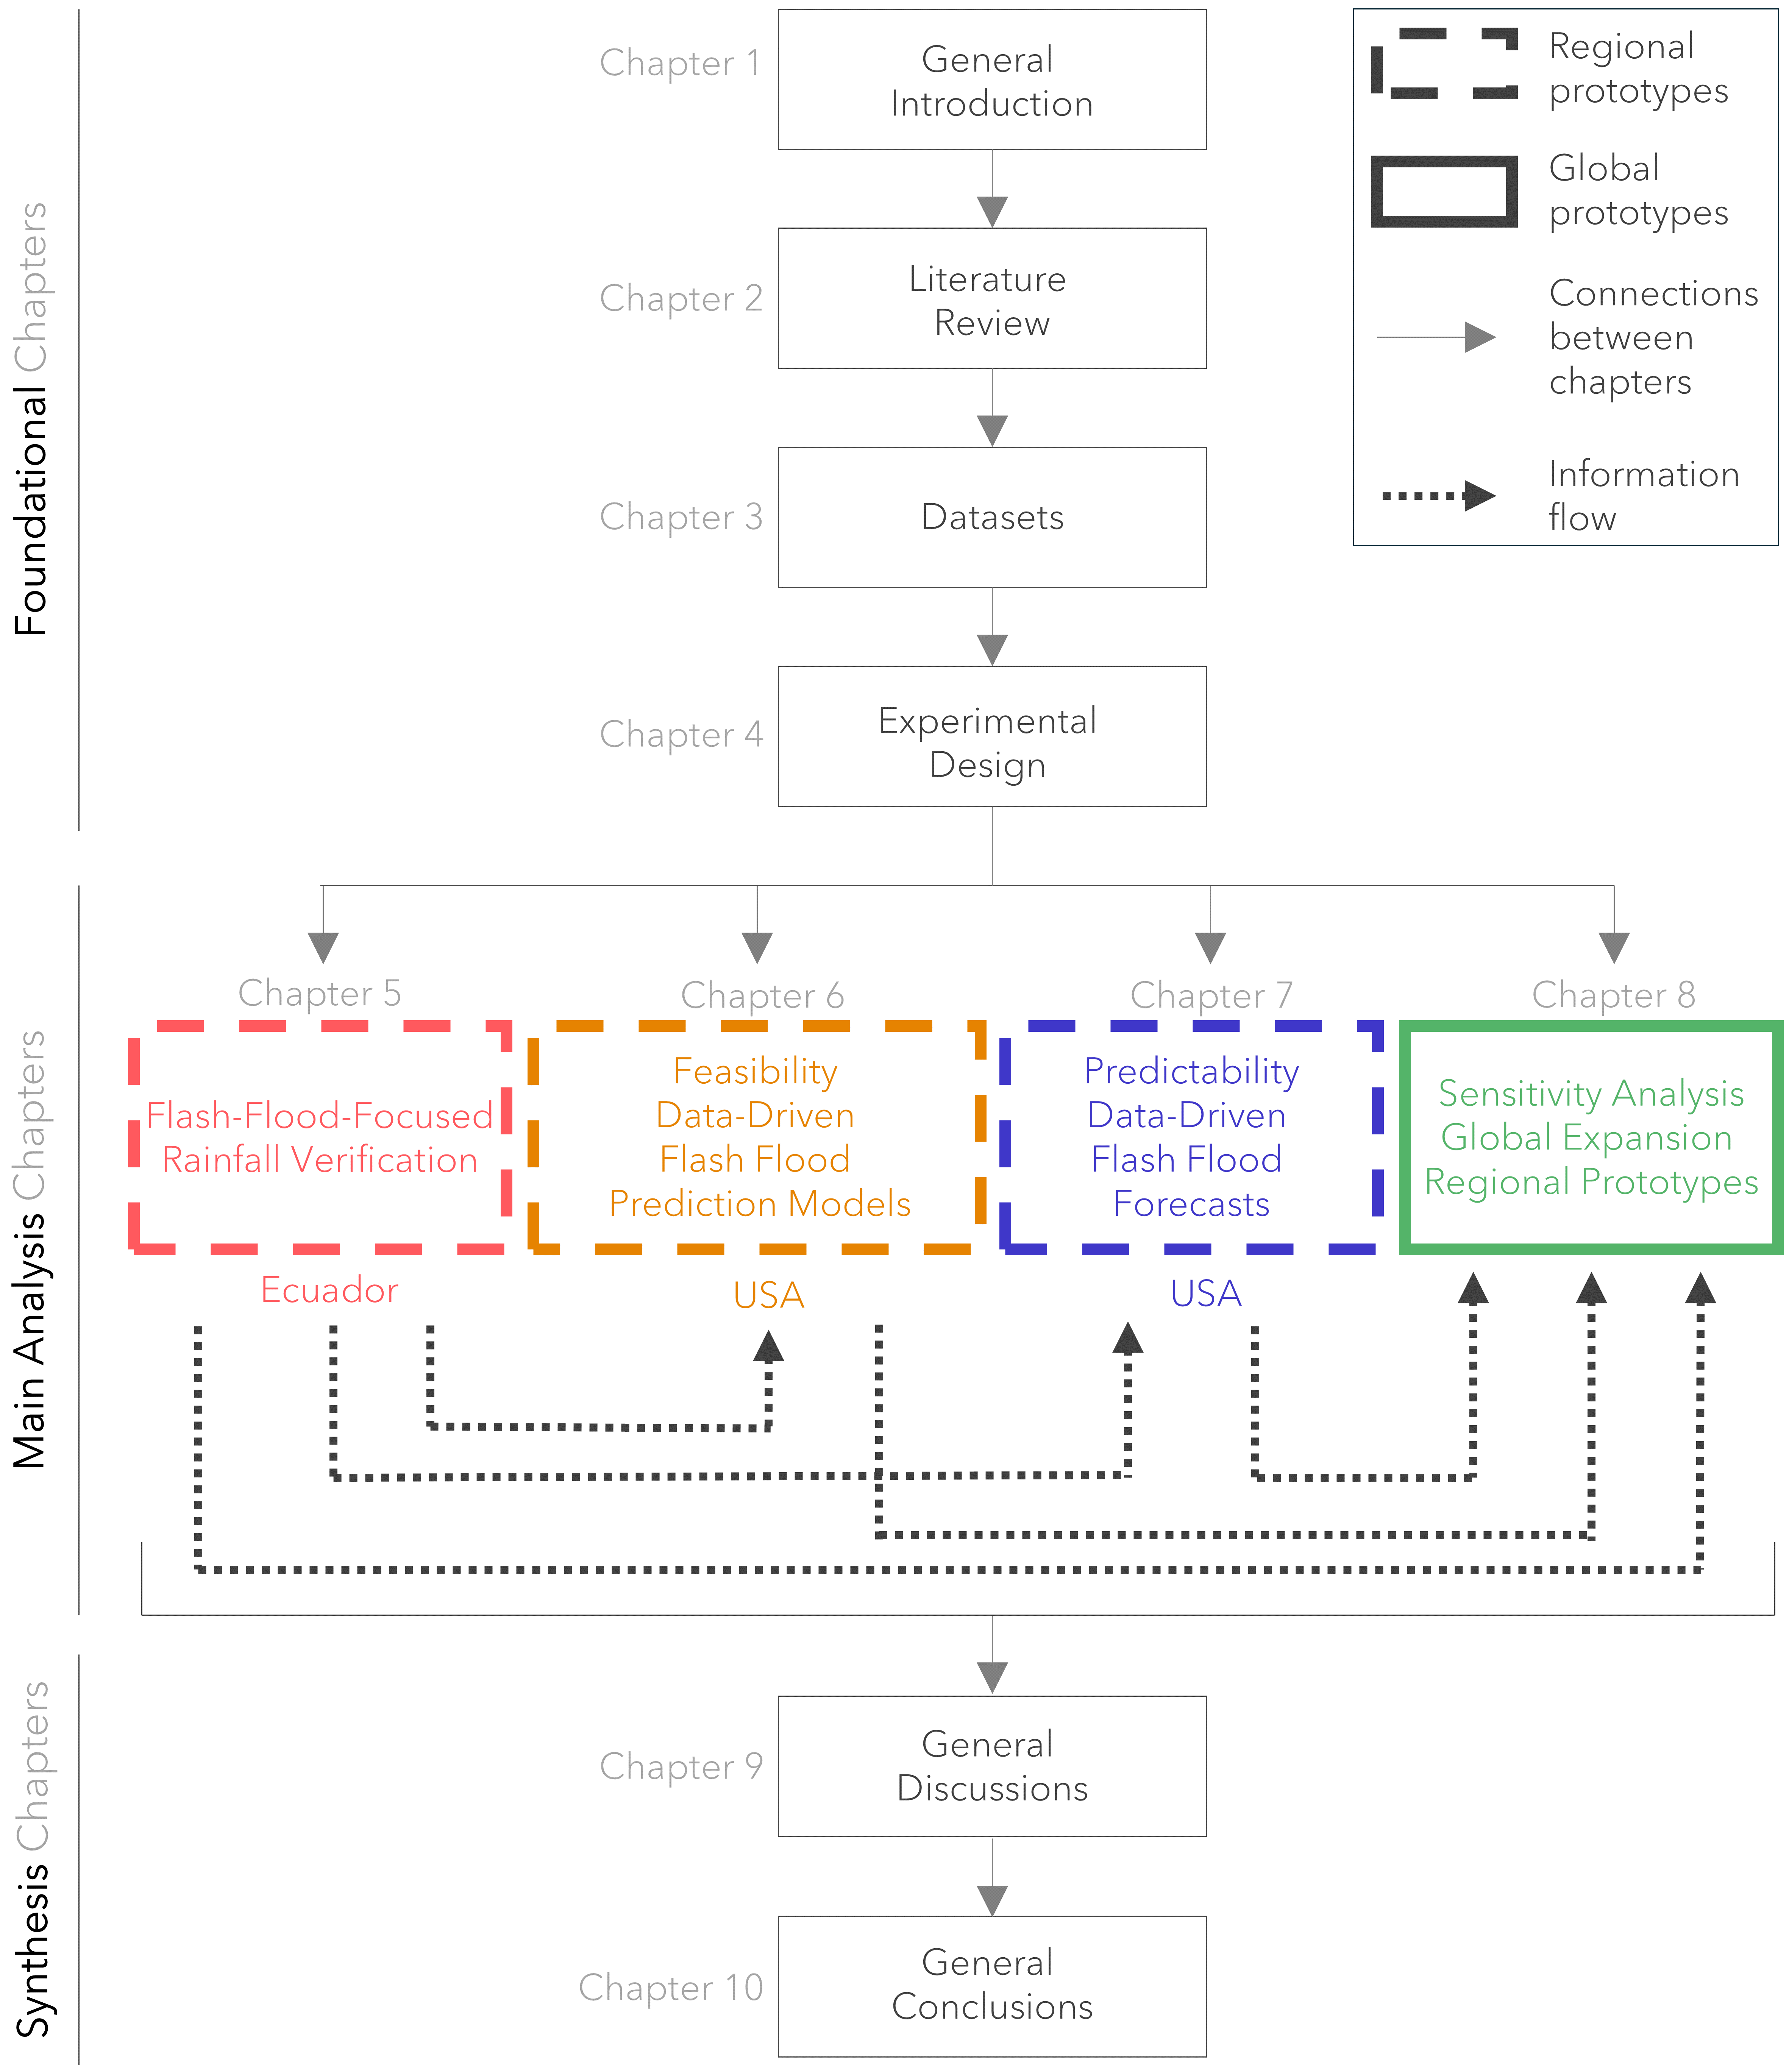
\includegraphics[width=\textwidth]{Figures/Chapter_01/01_thesis_roadmap.png}
\caption{\textbf{Overview of the thesis structure.} It illustrates the progression from the \textit{Foundational Chapters} (General Introduction - Chapter 1; Literature Review - Chapter 2; Datasets - Chapter 3; Experimental Design - Chapter 4), followed by the \textit{Main Analysis Chapters} (Flash-Flood-Focused Rainfall Verification - Chapter 5, indicated in pink; Feasibility of Data-Driven Flash-Flood Prediction Models - Chapter 6, indicated in yellow; Predictability of Data-Driven Flash-Flood Forecasts - Chapter 7, indicated in blue; Sensitivity analysis for global expansion of regional prototypes - Chapter 8, indicated in green), and concluding with the \textit{Synthesis Chapters} (General Discussions - Chapter 9; General Conclusions - Chapter 10).}
\label{fig:thesis_structure}
\end{figure}

\textbf{Chapter 1} \marginpara{Foundational Chapter - General Introduction} established the foundation for this research by addressing the critical need for improved flash flood early warning systems worldwide. It examined current limitations in verifying rainfall forecasts from global NWP models for flash flood applications and introduced the promising potential of data-driven approaches for flash flood prediction. The chapter presented three interconnected research questions focusing on developing new verification frameworks for flash-flood-focused verification of global NWP rainfall forecasts, creating data-driven flash flood prediction models using reanalysis data, and analysing the predictability of such forecasts to medium-range lead times.

\textbf{Chapter 2} \marginpara{Foundational Chapter - Literature Review} presents a comprehensive literature synthesis that establishes the scholarly foundation for the thesis's original contributions. The chapter begins by examining the fundamental concepts in flash flood prediction. It then critically evaluates the capabilities and limitations of global NWP models in generating rainfall forecasts suitable for flash flood applications, identifying key performance gaps. The review 
also traces the evolution from traditional flash flood prediction approaches to emerging data-driven techniques, highlighting significant advances and persistent challenges in predicting flash floods at a global scale.

\textbf{Chapter 3} \marginpara{Foundational Chapter - Datasets} presents and examines the essential datasets underpinning the development of flash-flood-focused verification frameworks for global NWP rainfall forecasts and data-driven flash flood prediction systems. It presents the rainfall datasets considered from raw and post-processed global NWP models and reanalysis. It also presents the orographic and hydrological parameters characterising terrain, soil and vegetation conditions preceding flash flood events. The chapter finally presents the flash flood impact databases (regional and global) used throughout this thesis, discussing their geographical coverage, temporal resolution, and inherent reporting limitations. 

\textbf{Chapter 4} \marginpara{Foundational Chapter - Experimental Design} establishes the thesis's methodological framework, demonstrating the strategic interconnection between research questions. The flash-flood-focused verification of global NWP rainfall forecasts forms the foundation that informs subsequent research stages by revealing their capabilities in predicting flash flood events at short- and medium-range lead times. The development of data-driven models using reanalysis data serves as the essential second stage, creating the predictive architecture subsequently employed to create the medium-range data-driven flash flood forecasts and establishing the performance benchmark against which such forecasts will be evaluated. 

\textbf{Chapter 5} \marginpara{Main Analysis Chapter - Flash-Flood-Focused Rainfall Verification}
introduces a robust flash-flood-focused verification methodology to evaluate global NWP rainfall forecasts' performance in identifying flash flood risk areas, contributing to answer RQ1. The chapter focuses on Ecuador, where a detailed impact database exists. The methodology directly verifies rainfall forecasts against flash flood impact observations, addressing challenges like interpreting metrics for dissimilar quantities and managing unreported events. Long-term objective verification and case studies validate the framework while revealing the strengths and limitations of global NWP rainfall forecasts for flash flood prediction. 

\textbf{Chapter 6} \marginpara{Main Analysis Chapter - Feasibility of Data-Driven Flash Flood Prediction Models} examines the feasibility of developing data-driven flash flood prediction models using global ERA5 hydro-meteorological reanalysis data. The research presents innovative data-driven architectures designed to process ERA5 hydro-meteorological data, carefully considering predictor selection, training strategies, and uncertainty assessment methodologies. Utilising NOAA's Storm Event Database over the contiguous US, the models undergo rigorous validation through both objective score-based verification and subjective case-study analysis following the flash-flood-focused verification framework developed in Chapter 5. The chapter further explores the models' transferability to different geographical regions and climate conditions through sensitivity analyses.

\textbf{Chapter 7} \marginpara{Main Analysis Chapter - Predictability of Data-Driven Flash Flood Forecasts} assesses the predictability of data-driven flash flood forecasts up to medium-range lead times, using ERA5 hydro-meteorological forecasts, and following the flash-flood-focused verification framework developed in Chapter 5. Building on the data-driven flash flood prediction model developed in Chapter 6, this investigation addresses the challenges of utilising forecast data, including prediction uncertainty and reliability across various lead times through objective verification and case studies. 

\textbf{Chapter 8} \marginpara{Synthesis Chapter - General Discussions} synthesises and discusses the research findings in the main analysis chapters, critically evaluating how effectively each research question was addressed. The chapter explores the broader implications for disaster risk reduction and emergency management, exploring how these advancements might enhance global early warning capabilities against impacts from flash floods. 

\textbf{Chapter 9} \marginpara{Synthesis Chapter - General Conclusions} concludes the thesis by articulating its novel contributions to flash flood prediction knowledge and practice. It provides final assessments for each research question, acknowledging methodological limitations whilst clearly stating the scientific advancements achieved. The chapter concludes by exploring future research directions that might strengthen the use of forecasts from global NWP models and data-driven approaches for predicting flash floods over a continuous global domain up to medium-range lead times. 